\documentclass[journal]{./IEEE/IEEEtran}
\usepackage{cite,graphicx}

\newcommand{\SPTITLE}{Sales and Inventory Management System for a Pawnshop Business}
\newcommand{\ADVISEE}{Azha Vianca de Belen}
\newcommand{\ADVISER}{Roinand Aguila}

\newcommand{\BSCS}{Bachelor of Science in Computer Science}
\newcommand{\ICS}{Institute of Computer Science}
\newcommand{\UPLB}{University of the Philippines Los Ba\~{n}os}
\newcommand{\REMARK}{\thanks{Presented to the Faculty of the \ICS, \UPLB\
                             in partial fulfillment of the requirements
                             for the Degree of \BSCS}}
        
\markboth{CMSC 190 Special Problem, \ICS}{}
\title{\SPTITLE}
\author{\ADVISEE~and~\ADVISER%
\REMARK
}

\pubid{\copyright~2017~ICS \UPLB}


%%%%%%%%%%%%%%%%%%%%%%%%%%%%%%%%%%%%%%%%%%%%%%%%%%%%%%%%%%%%%%%%%%%%%%%%%%

\begin{document}

% TITLE
\maketitle

% ABSTRACT
\begin{abstract}
A Sales and Inventory Management System for Small-Scale Pawnshop Business was developed using PHP language, CodeIgniter framework, PostgreSQL database, Apache2 server and MaterializeCSS. This project was developed to help the small-scale pawnshop owners in tracking and monitoring their inventory and sales.It aims to handle all the transactions of the business effficiently and effectively.
\end{abstract}


% INDEX TERMS

% INTRODUCTION
\section{Introduction}

\subsection{Background of the Study}
An inventory is a complete list of stock of some kind of physical commodity and total stocks of various kinds of a firm. It is the quantity of the product that is available to be sold by a merchandising firm at any given time. But  inventory does not only refer to physical merchandise. It can also refer to available seats on flights (airline passsenger reservation system) or slot availability in each class (university/college registration system). \cite{anigbogu11}

An inventory management system, on the other hand, monitors the quantity of available products for sale and maintanance of proper stock levels. It is very convenient for wholesale and retail stores (like the supermarkets) and other businesses to use this kind of system. It can facilitate the management and decision of sales, thus reducing the burden of the business and its managers. \cite{ren13} Also, the work efficiency can be improved as it lessens time and effort of the employees as well as the human errors from manual counting and recording. \cite{rajeswari16} Using an effective and efficient inventory management system is very critical to the over all performance and profitability of many businesses.

Sales and inventory management systems are common nowadays. A lot of sales and inventory managem ent systems were developed for the past years. They have been used in different businesses (especially the big ones) for competitive advantages and for efficiency and effectiveness of the business. Developing it for small-scale and medium-scale businesses will help them improve their operations, management and performance.

\subsection{Significance of the Study}
There are a lot of pawnshops in the Philippines but not all of them uses a management system to handle all their transactions. Most of them, especially the small-scale and medium-scale pawnshop businessess, still transacts with their clients and monitor their sales and inventory manually.This consumes a lot of time and effort for the pawnshop owners and their staff.

The purpose of the project is to create a system that will handle the transactions of a medium-scale pawnshop business like J and M pawnshop. The system will also track and monitor their inventory and sales and generate sales and inventory reports automatically. This will help the pawnshop owners to manage their business efficiently and effectively.

The system will make the transaction easier and secured for both the client and the pawnshop owner. All transaction records will be safe once these are encoded and stored in the database system. The system will have a good password encryption to protect all of its data. Only the administrator and staff with registered account can access the system. It will also be easier for the pawnshop owner (administrator) to generate the Sales and Inventory reports since all computations will be automatically computed based on the database  records. 

The system will also have an SMS Notification Feature. It will be easier for the administrator to notify their clients about their transaction details (like deadline of payment) and other announcements. 

\subsection{Objectives}
Generallly, the objective of he project is to develop a system that will cater to the needs of the medium-scale pawnshop business like J and M Pawnshop. It aims to help the pawnshop owner and administrators to easily monitor their inventory and sales and also to efficiently manage their transactions with their clients.

Specifically, the project aims to accomplish the following objectives:

1. To develop a system that will monitor the inventory and sales of a medium-scale pawnshop business;

2. To automatically generate the sales and inventory reports;

3. To develop an SMS Notification Feature that will be used to notify the clients; and

4. To develop an effective and efficient protocol in handling the business transactions and records.

\subsection{Scope and Limitations}
The system will consist of significant features/modules that will satisfy the business’ needs. These includes the Transaction, Inventory and Sales Modules. There will only be two kind of users (the administrator and the staff) who can use the system. The access will be limited depending on the user/account type. Customers/guest cannot access the system. 

The staff can only View/Update his profile. He can also Add/View/Update/Delete/Search transactions and View/Search list of Admins and Staff. The administrator can do the all staff's functionalities. In addition, he can also Add/Update/Delete list of administrator and staff, manage Sales and Inventory Records and view system logs. The administrator can also generate reports autoomatically. He can also send SMS notifications to customers but cannnot receive SMS from them.

% MATERIALS AND METHODS
\section{Review of Related Literature}
There are already a lot of inventory and sales management systems (and other related systems) that were created for the past years. For example, in the Institute of Computer Science (ICS) at the University of the Philippines Los Banos (UPLB), many students chose to create and develop systems for their Special Problem course. Those systems contributes in the idea of making this project.
	
In 2015, Ruel developed a similar system. She created an inventory and sales information system for a small-scale merchandising business that monitors the inventory and sales of the small grocery store. It also provides the users a conveniet way of handling the business transactions and records. It was implemented using PHP 5.5.12, HTML5, CodeIgniter 2.1.3, MySQL 5.6.17, Wamp Server 2.5 and Bootstrap 3.3.2.


Co (2012), as cited in Ruel’s paper, created an online accounting system a drug company. The system also monitors the inventory and sales of the company efficiently. Ruel also cited in her paper that Caraiga developed an Integrated  Sales and Inventory Management System that efficiently handles the transaction of a drugstore in 2005. \cite{ruel15}

In 2006, Cariño developed a Sales and Product Inventory Management Sytem for Leads Agricultural Product Corporation. The system was implemented using MicrosoftSQL Server 2000 and .NET Framework. I aimed to improve the efficiency and effectiveness of the business. \cite{carino11}

Implemented using PHP, Javascript, PostgreSQL, HTML, CSS and Yii Framewrok, Ong(2014), developed a Web-based Clinic Information and Inventory Management System. The sytem let the user view, add and update the medicines in the clinic. It also made the managing of records and inventory easier. \cite{ong14}
	
A similar system was also developed by San Buenaventura in 2014. He implemented Inventory of Supplies and Materials for Open LGU using Apache Web Server 2.2.22, PHP 5.4.3, Wappstack 5.4.19-0, PostgreSQL 9.0 and Yii 1.1.12. The system keeps track of all the incoming and outgoing resources of the departments. The user can add, view, update and delete supplies and materials. \cite{sanbuenaventura14}

% MATERIALS AND METHODS
\section{Materials and Methods}

\subsection{Materials}
The following were used to develop the User Interface, Database and Functionalities of the system:

-PHP 7.0

-Laravel Framework

-PostgreSQL

-Apache2 Server
 
-Bootstrap v3.3.7

-Chikka API

\subsection{Security Measures}
The user needs a registered account to access the system. They will be asked to put their username and password when logging in. Depending on his user/account type, the user will be directed to the home page after successfully logging in the system. 

Only the Administrator can add new Administrator and new Staff accounts. E
ach account will have be asked for a strong password. The system will require each user to have atleast an 8-character password with one number and one special character. The passwords will be encrypted using SHA1.

\subsection{System Functionalities}

\subsubsection{Administrator}
The following are the the administrator's functionalities.

-View/Update Profile

-Add/View/Update/Delete/Search Transaction

-Add/View/Update/Delete/Search list of administrator and staff

-Manage Sales and Inventory Records

-View/Generate Sales and Inventory Reports

-View Logs

-Send SMS Notification
	
\subsubsection{Staff}
The following are the the staff's functionalities.

-View/Update Profile

-Add/View/Update/Delete/Search Transaction 

-View/Search list of administrator and staff

\subsection{System Modules}

\subsubsection{Login}
The administrator and the staff can access the system using their registered account. The administrator can add new administrator and new staff.

\subsubsection{Home}
After logging in, the administrator or staff will be directed in this page. A summary of the inventory and sales records will be displayed 	in the administrator’s home page but not in the staff’s home page. It will also display the functionalities of the system depending on the account type.

\subsubsection{Administrators and Staff}
The list of the administrators and staffs (as well as their basic information) will be displayed in this page. The user can also 	add/view/update/delete/search administrator and staff depending on the account type.

\subsubsection{Transactions}
All the information about the transactions (as well as the actions that can be done with it) will be displayed in this page.

\subsubsection{Inventory}
The Inventory Record will be diplayed in this page. The Administrator can also generate the inventory report in this page.

\subsubsection{Sales}
Sales Record will be diplayed in this page. The Administrator can also generate the sales report in this page.

\subsubsection{SMS Notification}
The administrator and staff can send SMS notification to their clients in this page.

\subsubsection{About}
Information about the system will be displayed in this page.

\subsection{System Evaluation}
The client (administrators and staff) will be asked to use and test the system. A set of questionnaires will be given to evaluate the user-interface, functionalities and overall performance of the system. 

\subsection{Use Case Diagram}
\begin{center}

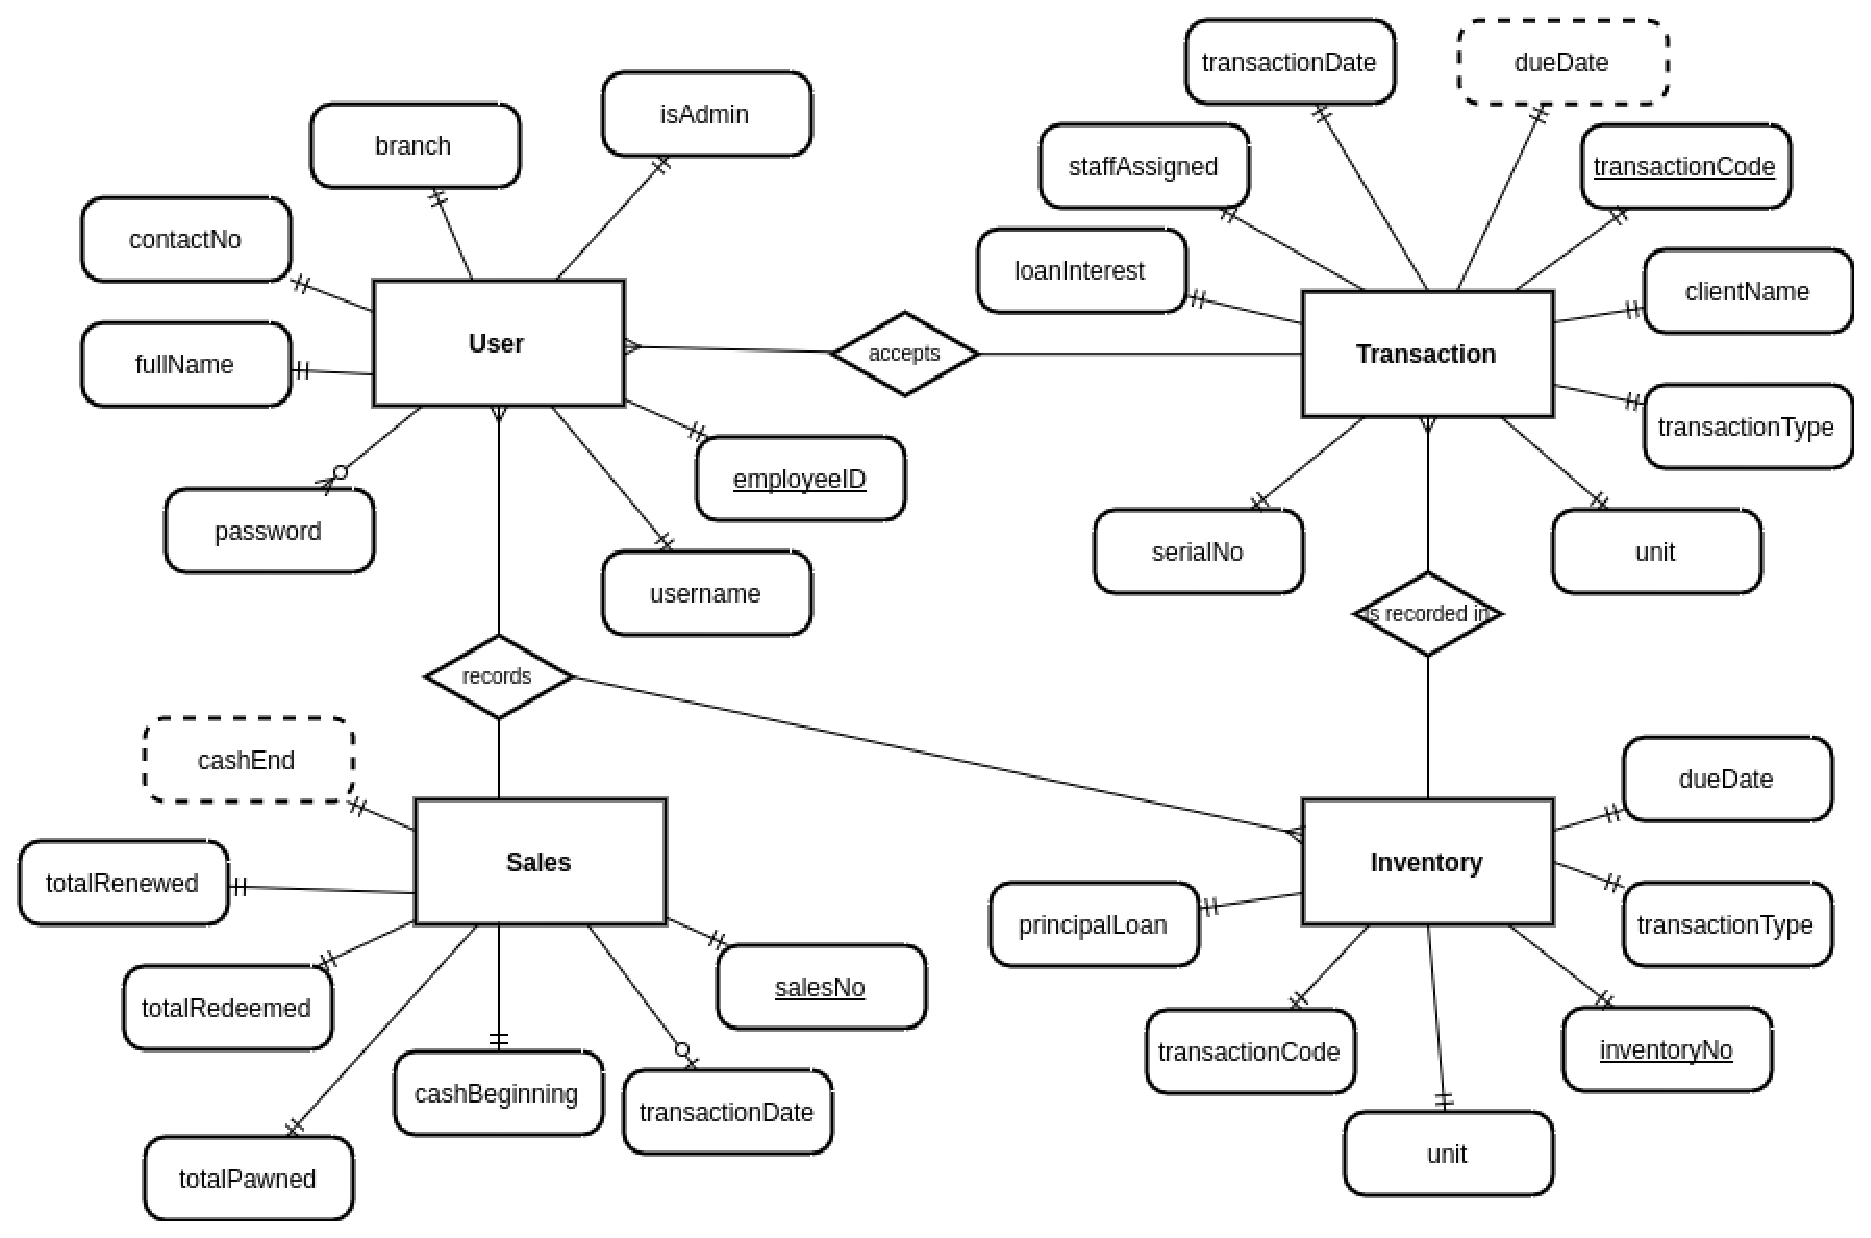
\includegraphics[height=60mm]{./images/erd.eps}

Figure 1. ERD

\end{center}

\subsection{Use Case Diagram}
\begin{center}

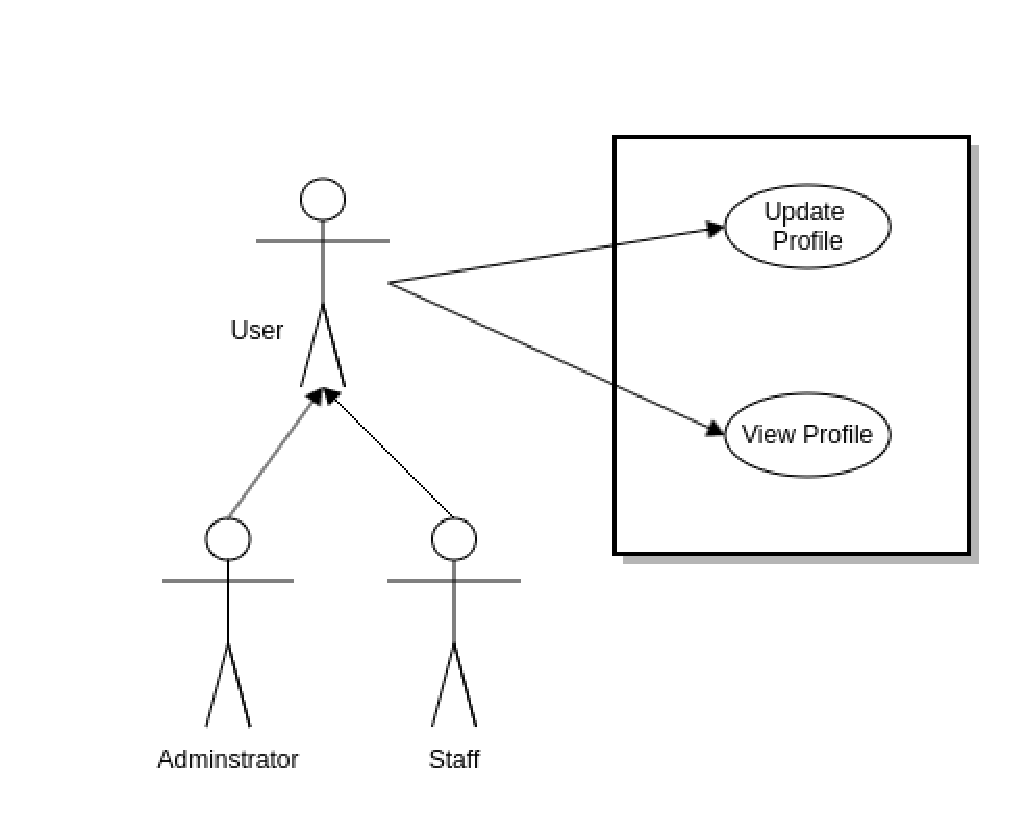
\includegraphics[height=60mm]{./images/useCase/profile.eps}

Figure 2. View/Update Profile

\includegraphics[height=60mm]{./images/useCase/adminstaff.eps}

Figure 3. Add/View/Update/Delete/Search Admin/Staff

\includegraphics[height=60mm]{./images/useCase/transaction.eps}

Figure 4. Add/View/Update/Delete/Search Transactions

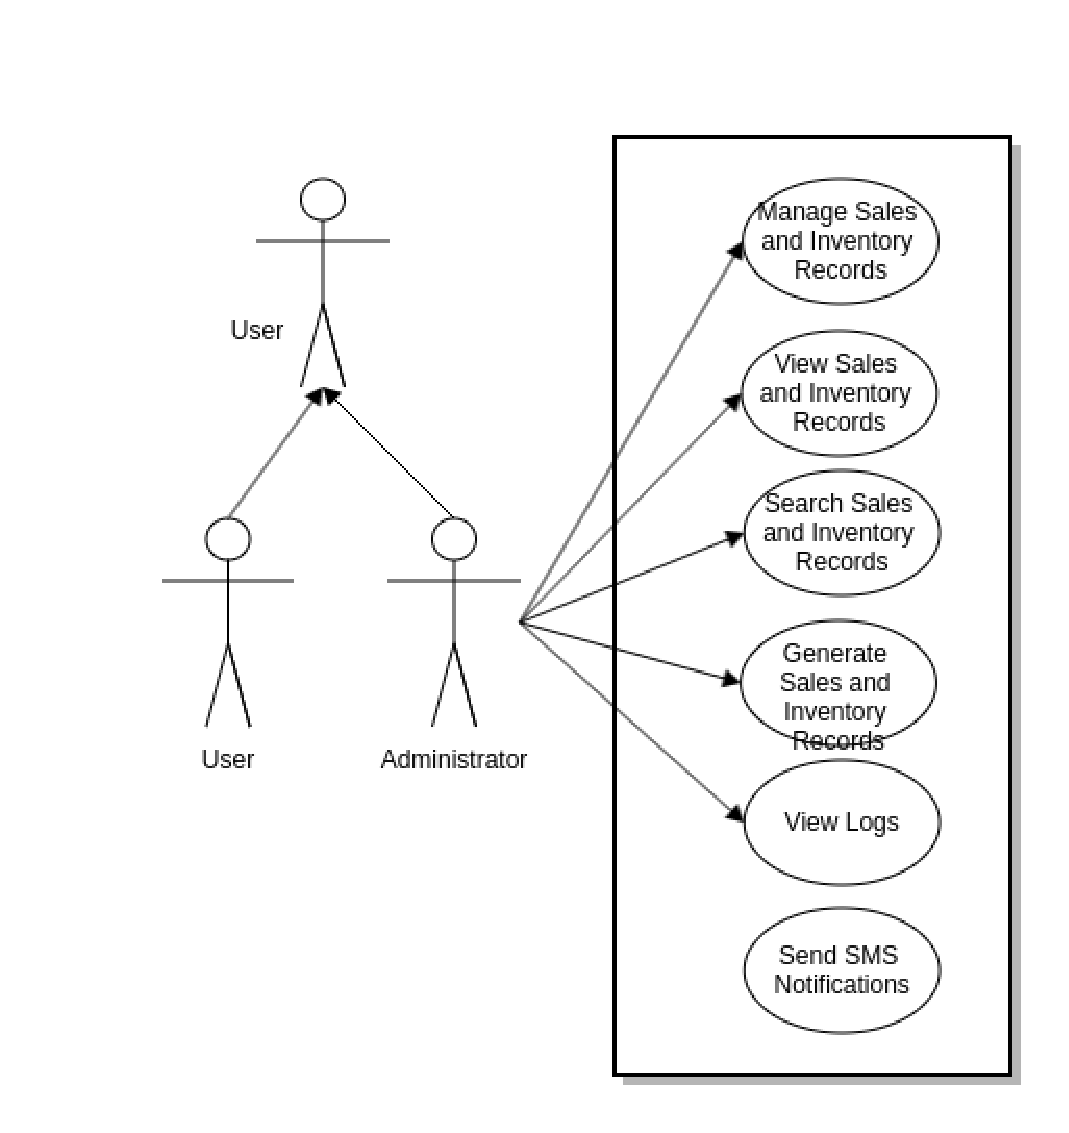
\includegraphics[height=60mm]{./images/useCase/salesinventory.eps}

Figure 5. Manage/View/Generate Sales and Inventory Records, View Logs, and Send SMS Notifications

\end{center}

\subsection{Mock-up UI}
\begin{center}

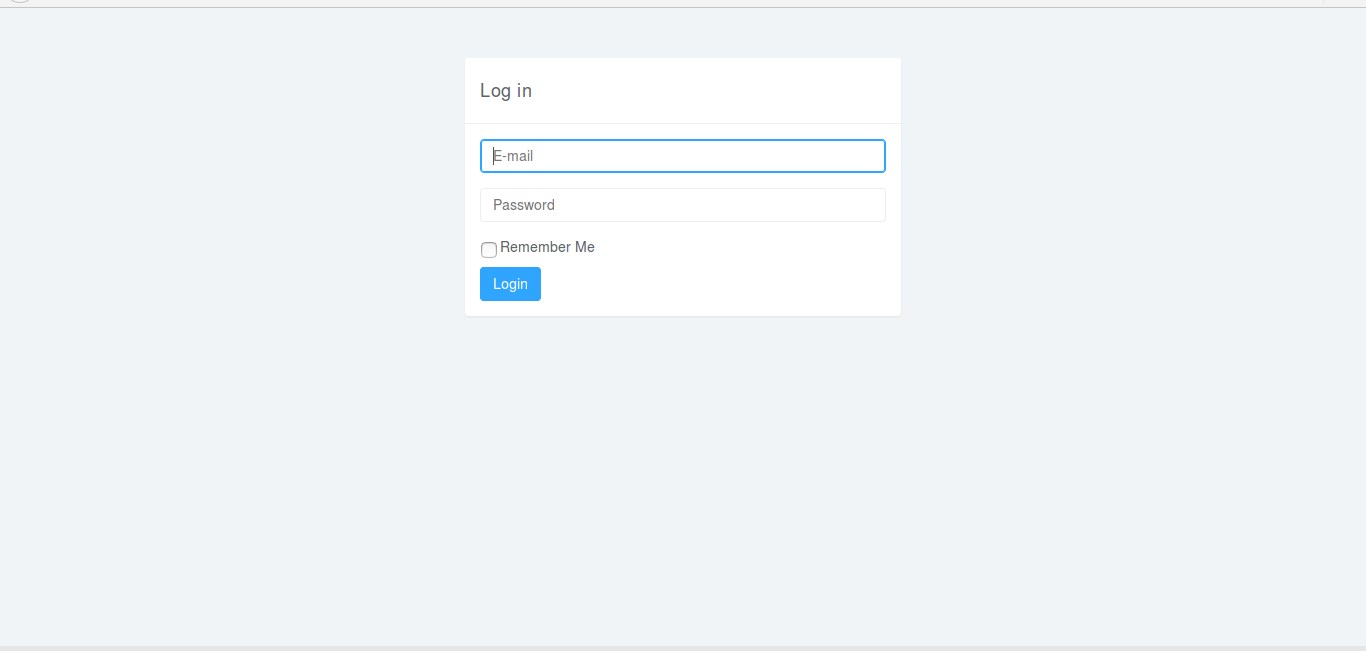
\includegraphics[width=80mm]{./images/mockupUI/login.eps}
Figure 6. Login Page


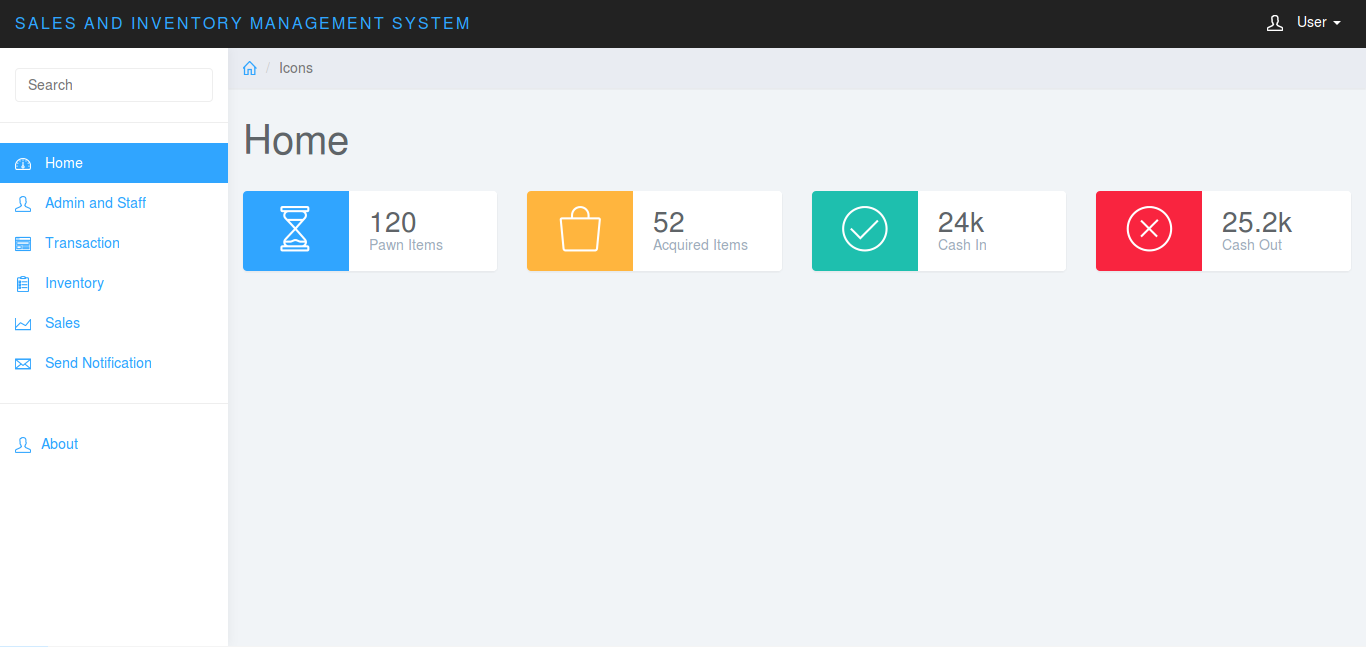
\includegraphics[width=80mm]{./images/mockupUI/home.eps}
Figure 7. Home Page


\includegraphics[width=80mm]{./images/mockupUI/adminstaff.eps}
Figure 8. Admin and Staff Page


\includegraphics[width=80mm]{./images/mockupUI/transaction.eps}
Figure 9. Transaction Page


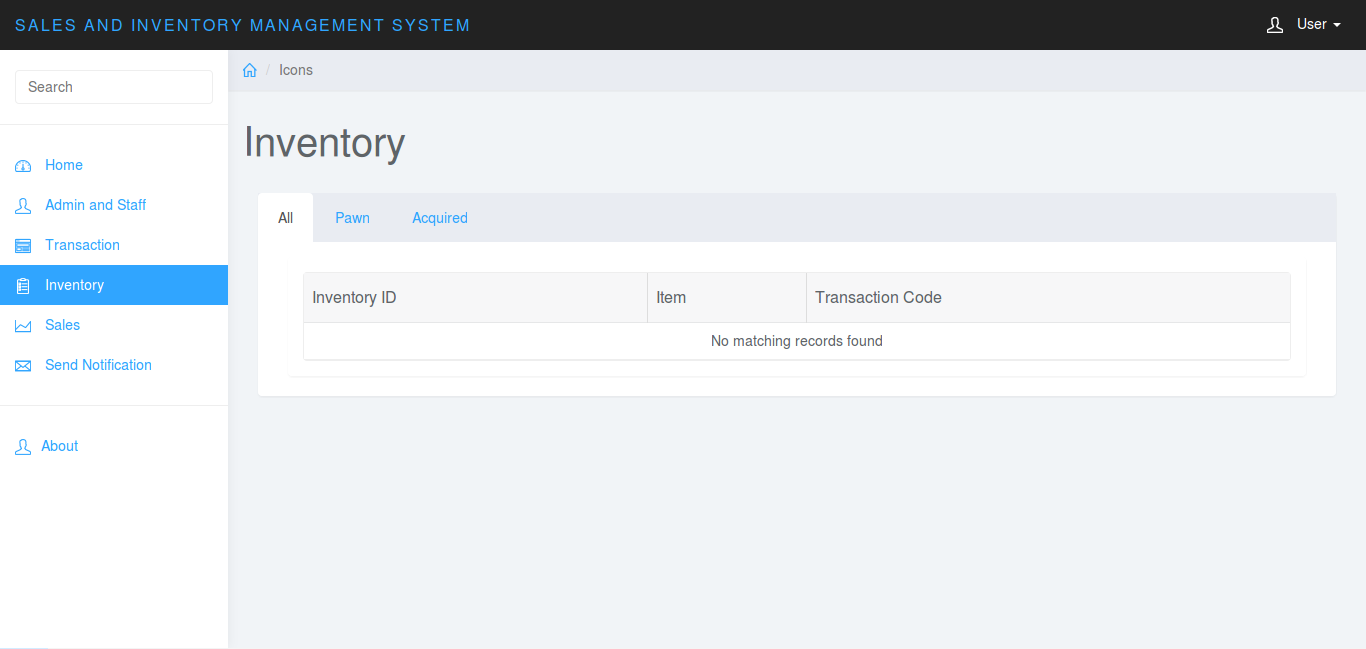
\includegraphics[width=80mm]{./images/mockupUI/inventory.eps}
Figure 10. Inventory page Page


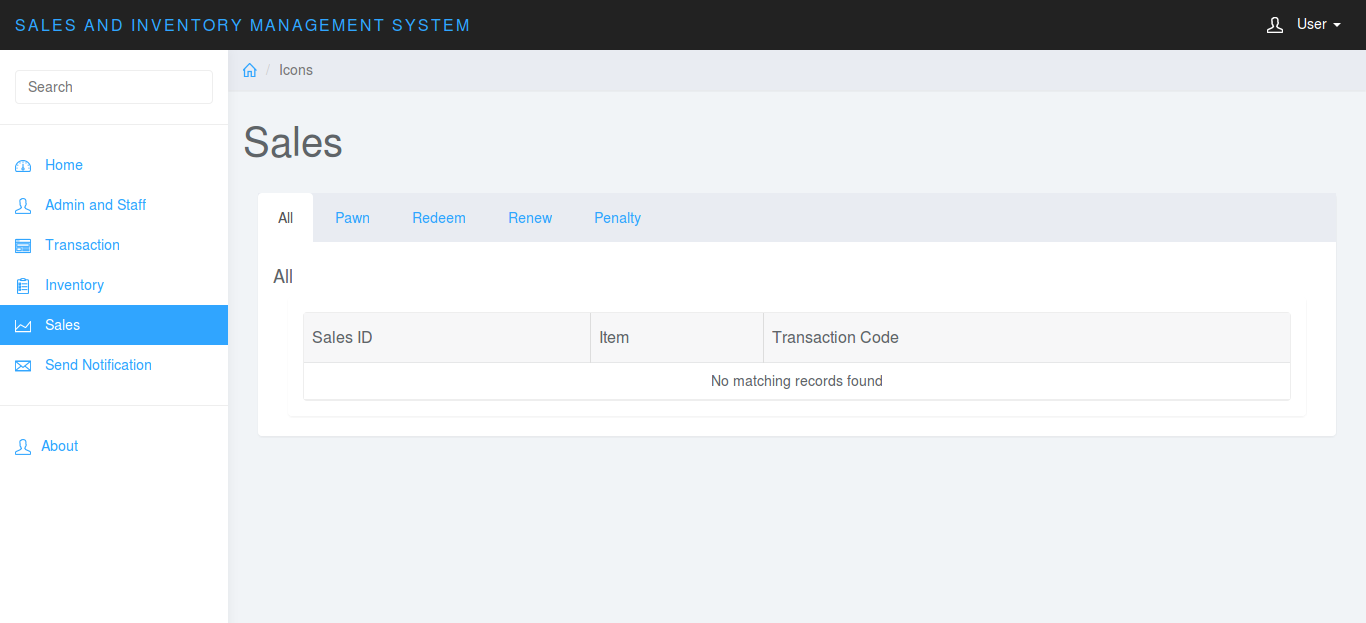
\includegraphics[width=80mm]{./images/mockupUI/sales.eps}
Figure 11. Sales Page


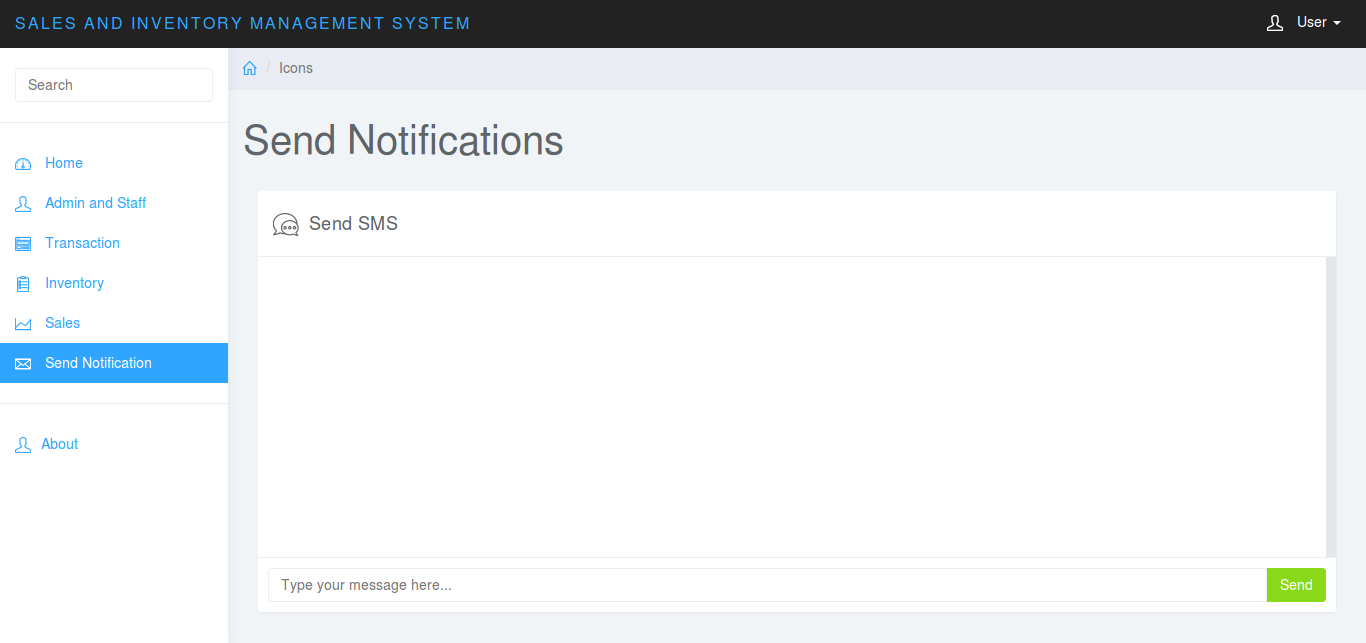
\includegraphics[width=80mm]{./images/mockupUI/sendnotif.eps}
Figure 12. Send SMS Notifications Page

\end{center}

% RESULTS AND DISCUSSION
\section{Results and Discussion}
The Sales and Inventory Management System (SIMS) was presented to the client, the manager of J and M Pawnshop. After the evaluation, the client felt satisfied with the system and its functionalities. The features such as monitoring transactions, generating reports in PDF and Excel, and sending SMS Notification satisfied the client. The Administrator can now track all their business transactions and generate reports and the Staff can handle the transactions efficiently using the system.

The system was developed using Laravel Framework, PostgreSQL database and Bootstrap. A Chikka API Package was used for the SMS Notification feature. The user interface was made simple and user-friendly for easier system navigation and usage.

For the evaluation of the system, the user was asked to rate the system from 1 to 10 (10 being the highest) using the following evaluatiion criteria:

-Overall impression of the system

-Understanding of the information asked in the forms

-User interface

-User friendliness/System Navigation

-User functionalities

-Generating reports

-Consistency of the system

-SMS Notification

% CONCLUSION AND FUTURE WORK
\section{Conclusion and Future Work}
The Inventory and Sales Management System can be used by pawnshop owners who still manually do and record their transactions. The system will help them in handlin their transactions well and keeping their records organized. 

The system is still open for other improvements and development. Additional functionalities can also be added to improve the system. A payroll system can also be integrated to the system's user module to organize the employees' payment.

% ACKNOWLEDGMENT
\section*{Acknowledgment}
Azha Vianca would like to thank her adviser, Sir Roi, for accepting her as his advisee and for allowing her to do this SP. She would like to thank her family for all their love and understanding and her roommates  and friends for their continuous support and encouragement while doing this system.  Above all, she wants to thank God for giving her the wisdom and guidance she needed to complete this requirement.


% BIBLIOGRAPHY
\bibliographystyle{./IEEE/IEEEtran}
\bibliography{./debelen-cs190-ieee}
% \nocite{*}

% BIOGRAPHY
\begin{biography}[{
\includegraphics[width=25mm]{./images/debelen.eps}}]{Azha Vianca N. de Belen}
Azha Vianca is the eldest daughter of Alfredo and Verijean de Belen. She is a proud volunteer of UPLB Pelikulab.
\end{biography}

 
\end{document}